
\section{\textcolor{black}{UQ and uncertainty types}} % Sections are added in order to organize your presentation into discrete blocks, all sections and subsections are automatically output to the table of contents as an overview of the talk but NOT output in the presentation as separate slides

%------------------------------------------------
\begin{frame}
\frametitle{What is Uncertainty Quantification (UQ)?}
\only<1>{\begin{quote}
    \Large All models are wrong, but some are useful.\\
    --George E.P. Box
\end{quote}
\bigskip

\hspace*{70pt} How inaccurate might the models be?\\
\hspace*{90pt}When are they useful in engineering problems?\\
\hspace*{110pt} How much confidence can we have in model's predictions?

\bigskip
\hspace*{130pt} \Large UQ provides a framework answering
\hspace*{140pt} these questions and making model useful.
}

\only<2>{
\begin{figure}
    \centering
    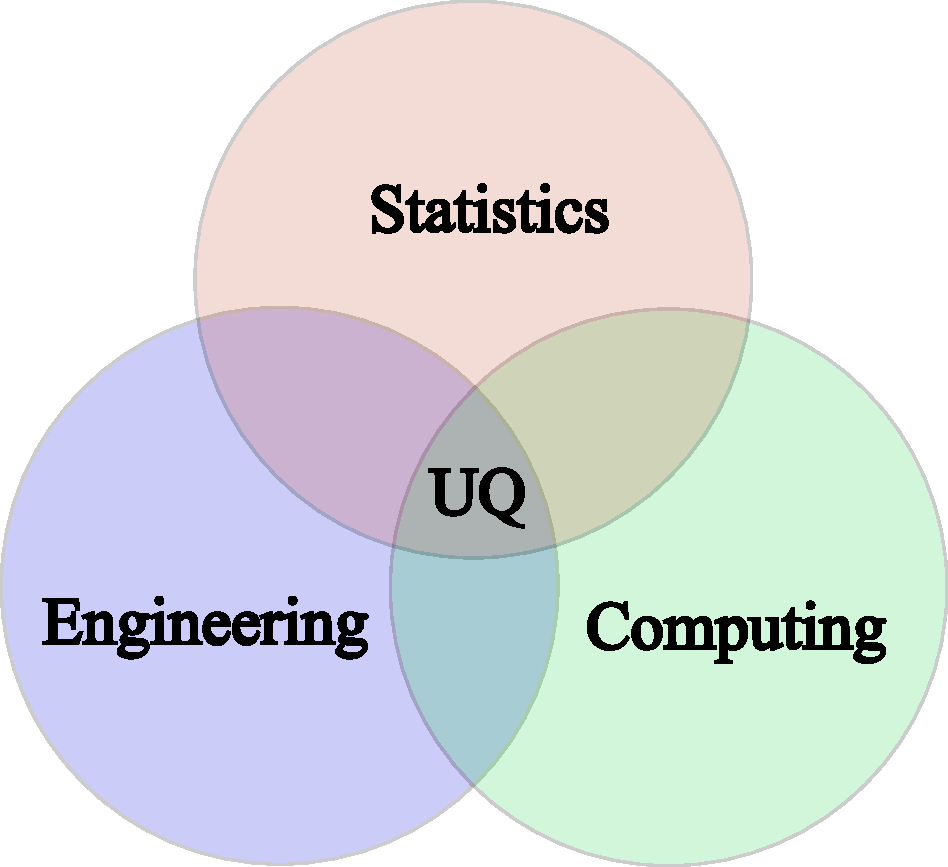
\includegraphics[width = 5.8cm]{figures/figure_UQ_subject.pdf}
    \label{fig:UQ-subject}
    \end{figure}

\begin{quote}
UQ is the science of quantitative \textcolor{red}{characterization} and \textcolor{red}{reduction} of uncertainties in both computational and real world applications\footfullcite{Saouma2021} 
\end{quote}
}



 \end{frame}
 %--------------------------------------------------------------------------------------------
 %-------------------------------------------------------------------

\begin{frame}
	\frametitle{Uncertain events in geotechnics}
    \begin{figure}
    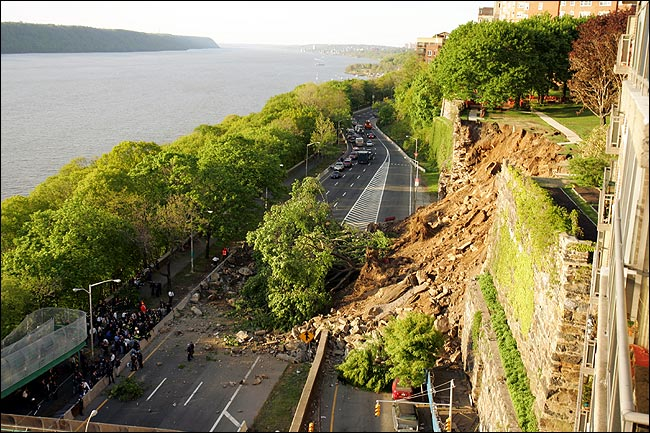
\includegraphics[height = 2.4cm]{figures/figure-geofailureone.jpg}    
    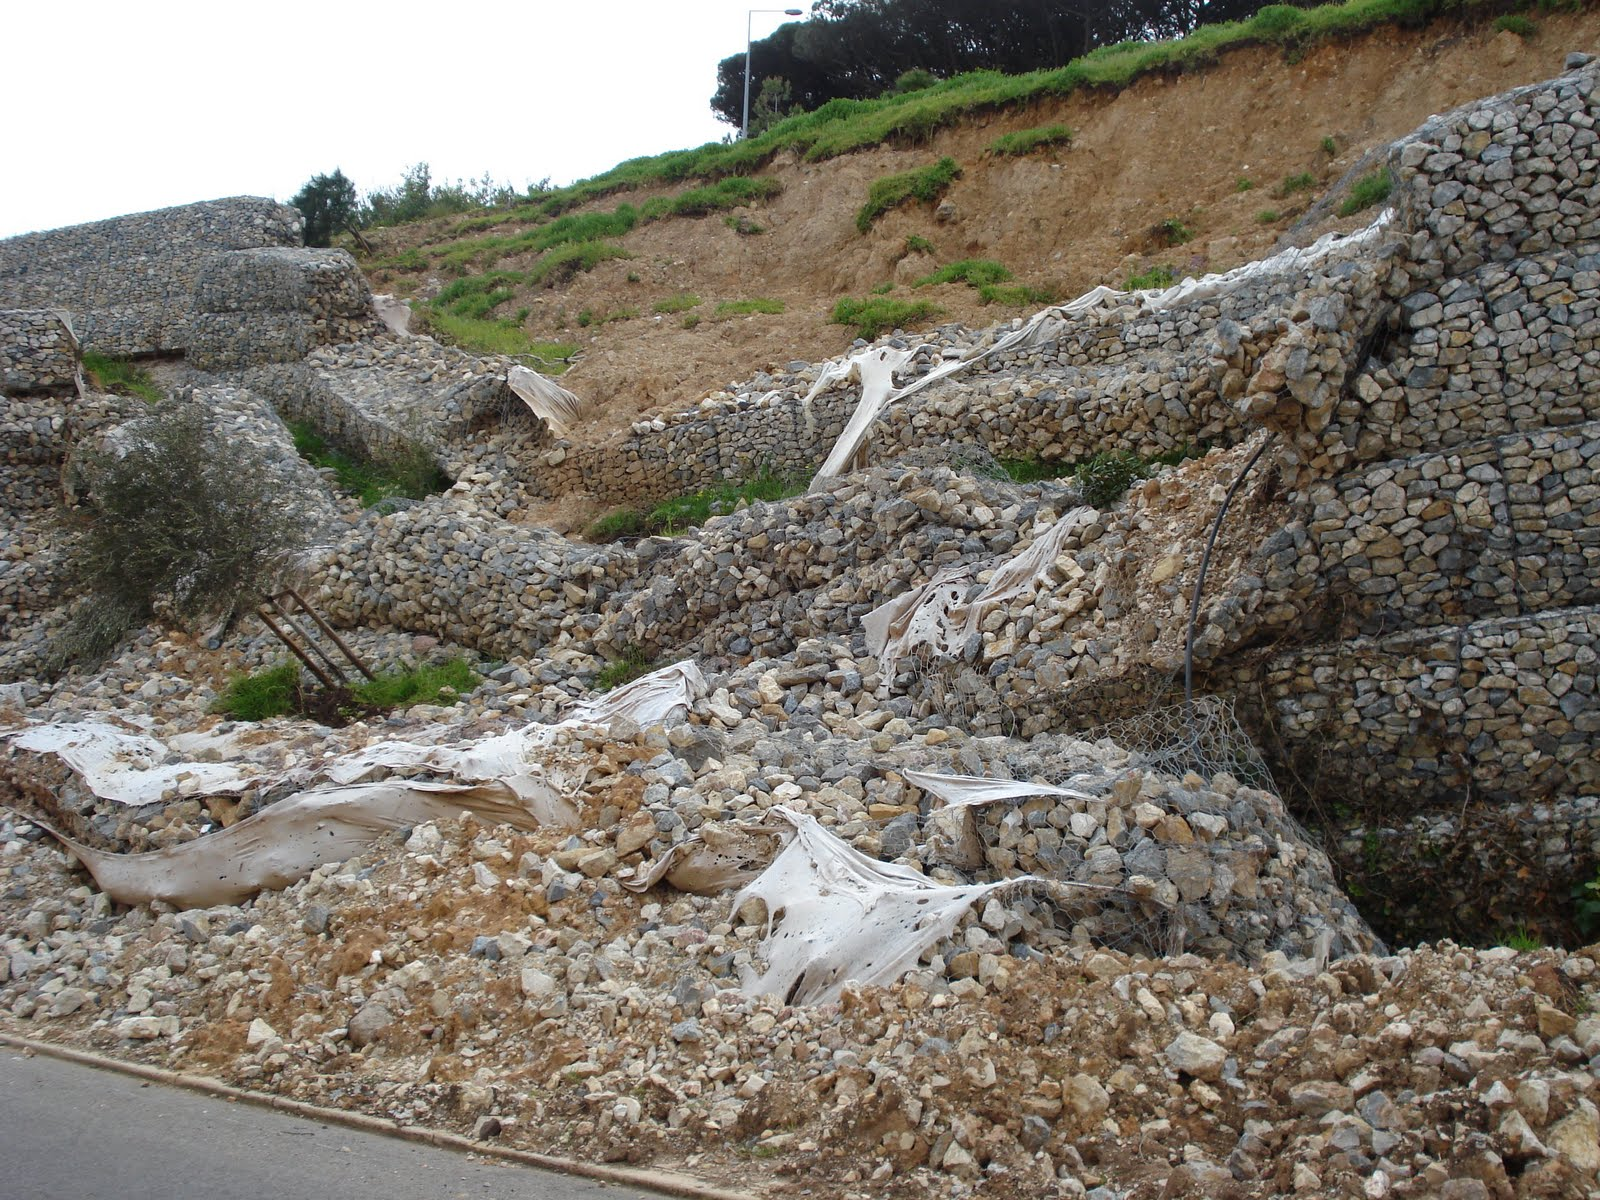
\includegraphics[height = 2.4cm]{figures/figure-geofailuretwo.jpg}  
    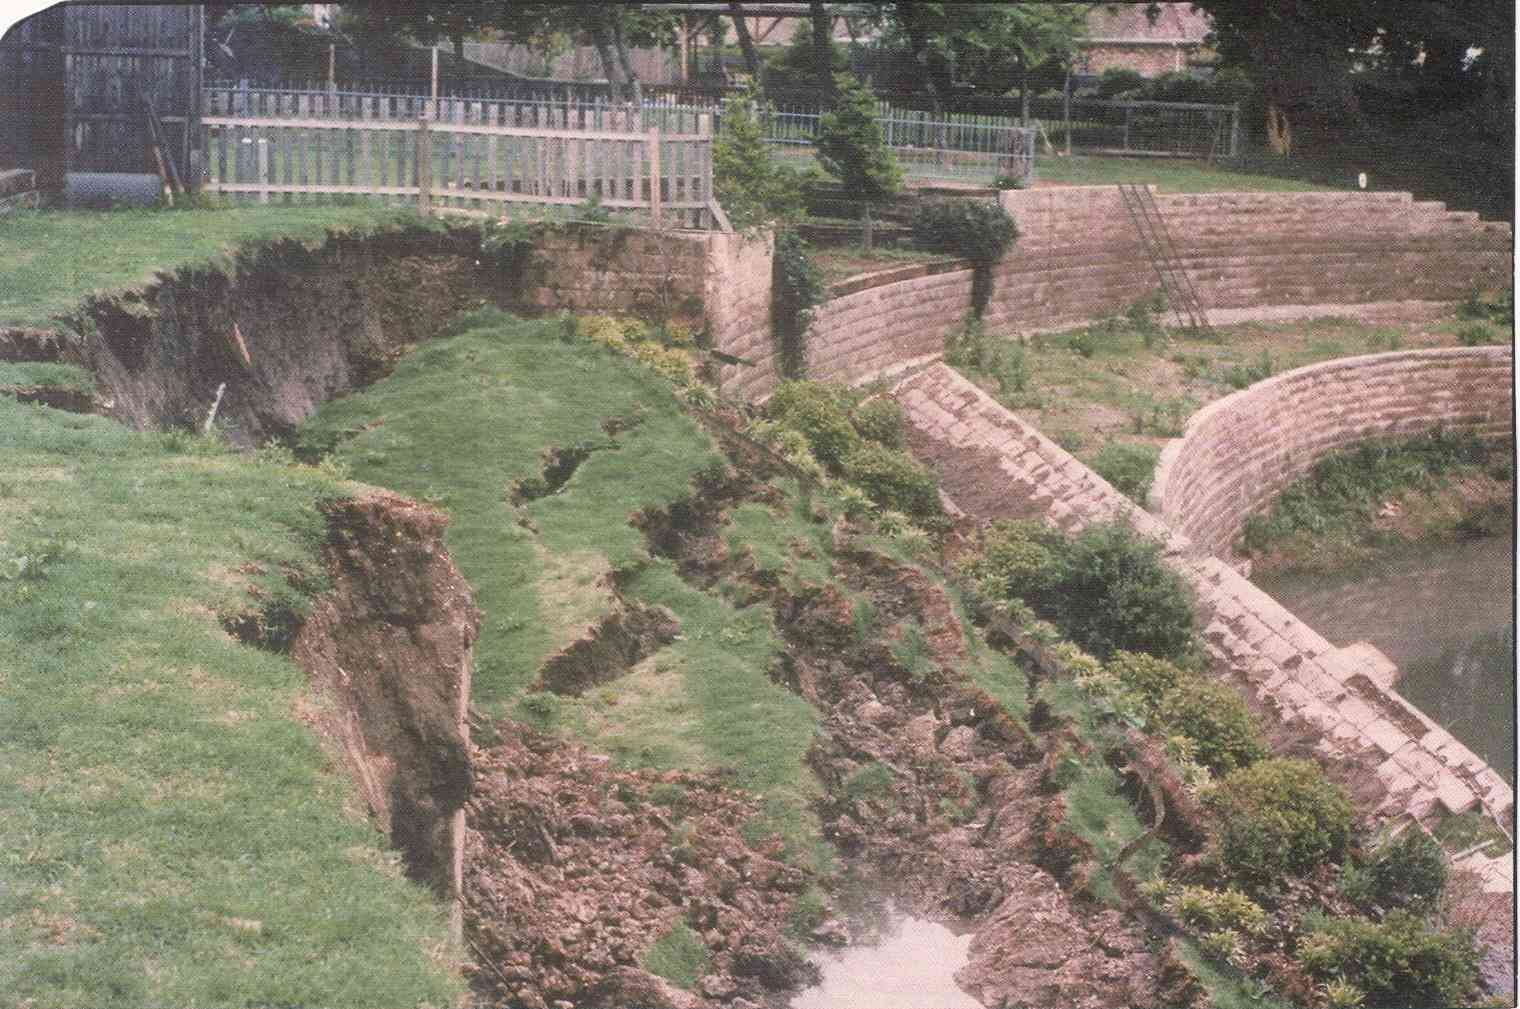
\includegraphics[height = 2.4cm]{figures/figure-geofailurethree.jpg}  
    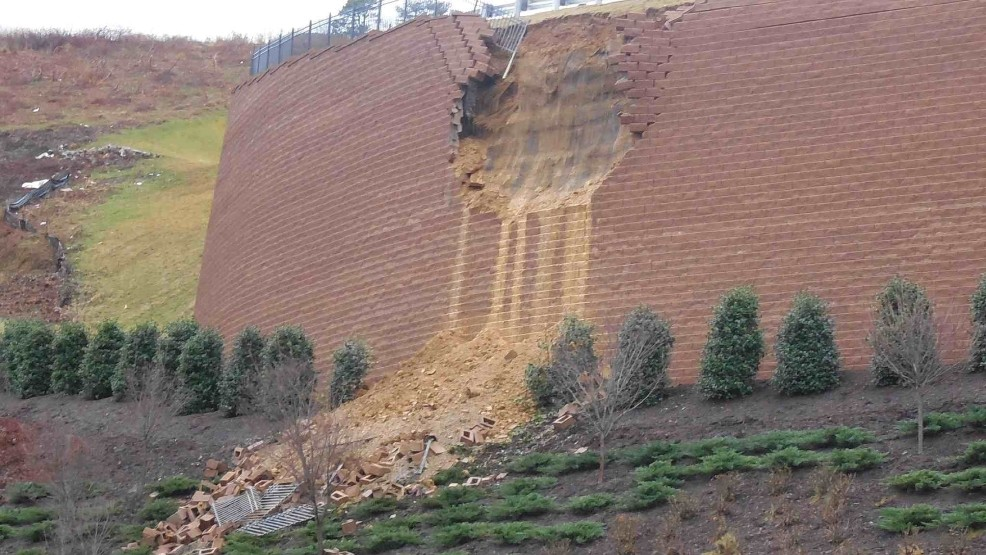
\includegraphics[height = 2.4cm]{figures/figure-geofailurefour.jpg}  
    \tiny\footnotetext{\href{https://www.capitalgeotechnical.com/geotechnical-failures.html}{capitalgeotechnical}}
    \end{figure}    
    
\end{frame}

%------------------------------------------------
\begin{frame}
\frametitle{Two types of uncertainties}
\framesubtitle{Aleatoric vs epistemic}

\begin{columns}
    \column{0.7\textwidth}
        \begin{figure}
        \centering
            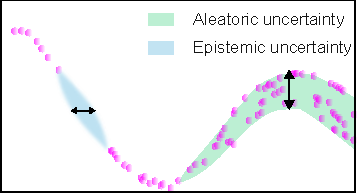
\includegraphics[width = 9cm]{figures/aleatoricvsepisidemic.pdf}
            \caption*{Aleatoric uncertainty vs Epistemic uncertainty}
        \end{figure} 
    \column{0.3\textwidth}
     \textbf{Distinguish}:
     \begin{block}{Aleatoric uncertainty}
statistical variability, inherently random effects (\textbf{irreducible})
     \end{block}
     \begin{block}{Epistemic uncertainty}
model uncertainty, a lack of knowledge (\textbf{reducible})
     \end{block}    
    \end{columns}
\end{frame}
%--------------------------------
\begin{frame}
\frametitle{Components of uncertainty :}
\Large\textbf{Total uncertainty $\approx$ aleatoric uncertainty $+$ epistemic uncertainty}
\begin{figure}
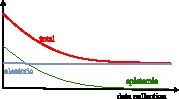
\includegraphics[scale=2.5]{figures/figure-total_Uncertainty.pdf}
\end{figure}

\end{frame}
%----------------------------------------------------------
\begin{frame}
\frametitle{Sources of uncertainties}
\framesubtitle{Mix of aleatoric and epistemic: Involve too much subjectivity}
\begin{figure}
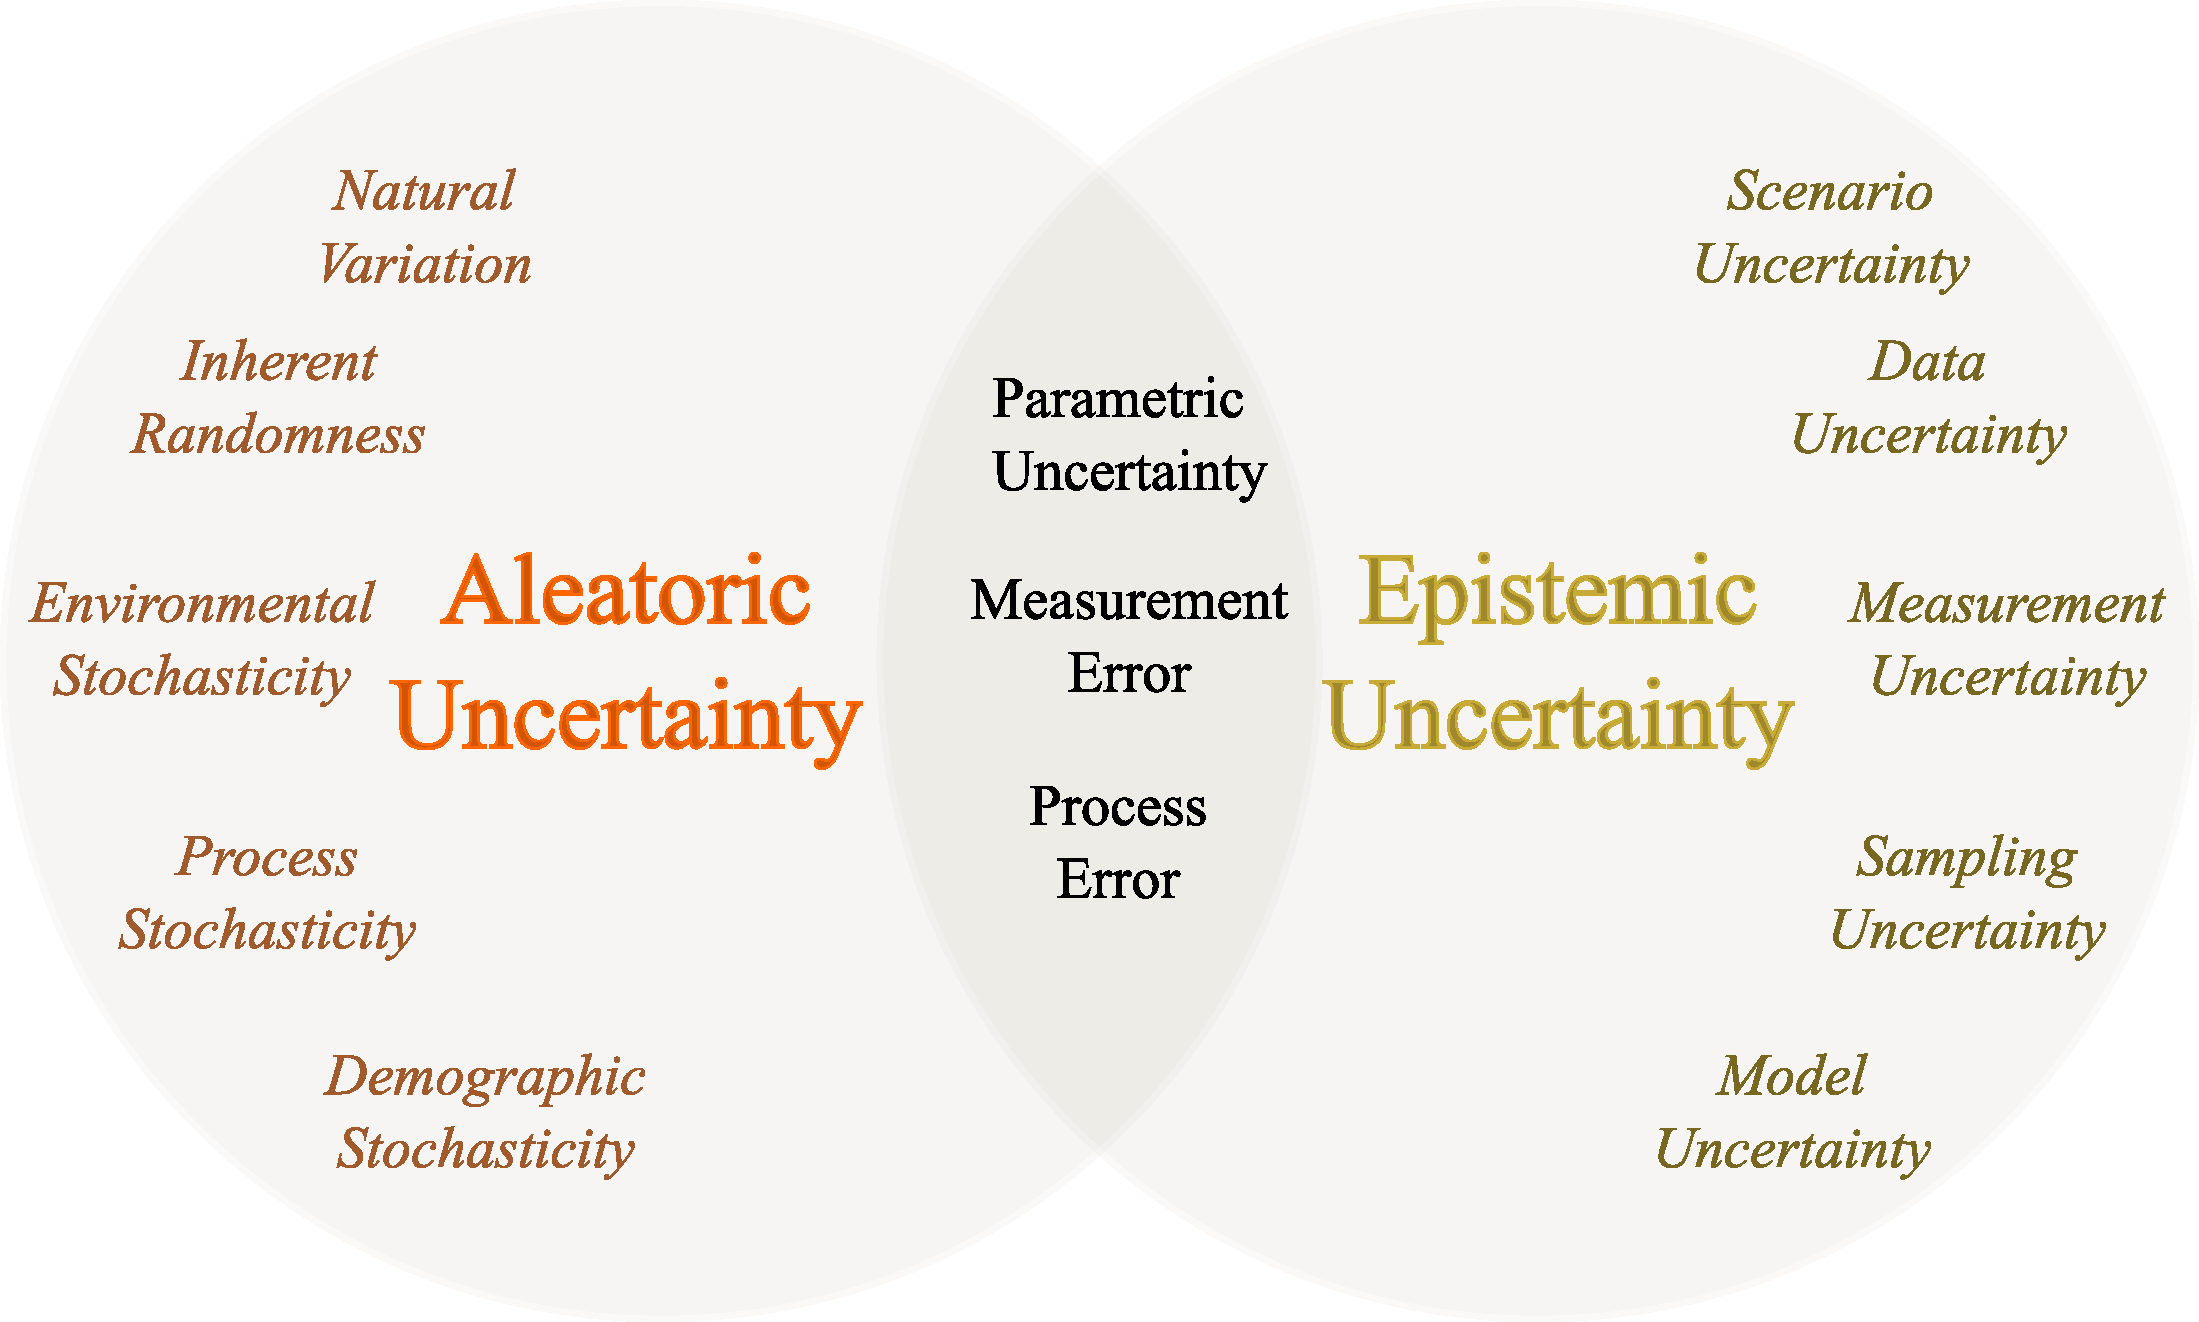
\includegraphics[scale=0.3]{figures/figure-uncertainty_classification.pdf}
\end{figure}
\end{frame}

%----------------------------------------------------------------------------
\begin{frame}
\frametitle{Examples}
    \begin{figure}
    \centering
    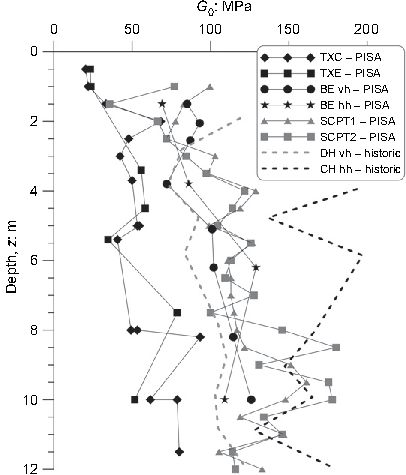
\includegraphics[scale=0.7]{figures/figure-UQtype2.pdf}
    \tiny\footcite{zdravkovic2020}
    \hspace{1cm}
    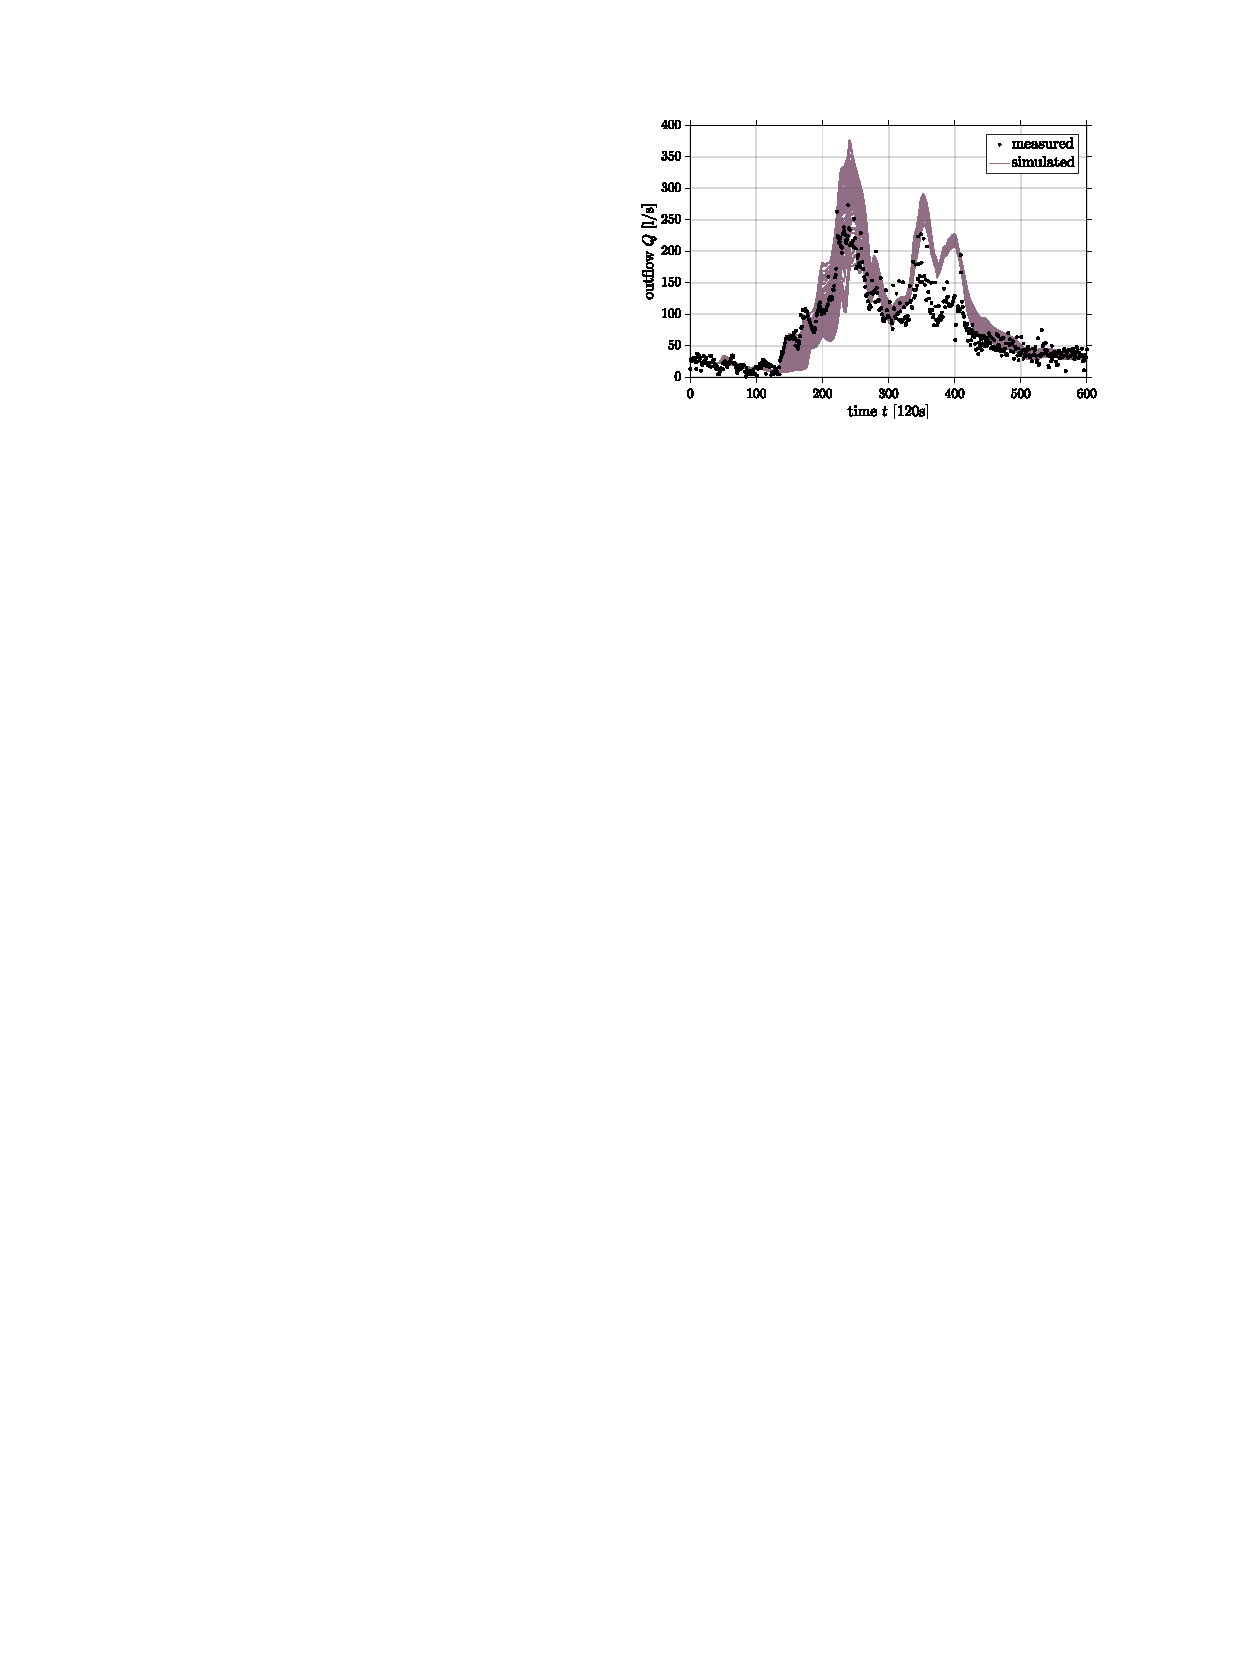
\includegraphics[scale=0.8]{figures/figure-UQtype3.pdf}
    \tiny\footcite{nagel2020}  
    \end{figure}
\end{frame}
